\documentclass{article}
\usepackage{fancyhdr}
\usepackage{extramarks}
\usepackage{amsmath}
\usepackage{amsthm}
\usepackage{amsfonts}
\usepackage{tikz}
\usepackage[plain]{algorithm}
\usepackage{algpseudocode}
\usepackage{multirow}
\usepackage{circuitikz}
\usepackage{amssymb}
\usetikzlibrary{automata,positioning,shapes.geometric, arrows.meta, calc}

% Custom Commands
\newcommand{\xmark}{%
\tikz[scale=0.23] {
    \draw[line width=0.7,line cap=round] (0,0) to [bend left=6] (1,1);
    \draw[line width=0.7,line cap=round] (0.2,0.95) to [bend right=3] (0.8,0.05);
}}
\newcommand{\cmark}{%
\tikz[scale=0.23] {
    \draw[line width=0.7,line cap=round] (0.25,0) to [bend left=10] (1,1);
    \draw[line width=0.8,line cap=round] (0,0.35) to [bend right=1] (0.23,0);
}}

% TikZ Styles
\tikzset{
    bus/.style={draw, thick, minimum width=2.5cm, minimum height=0.2cm}, 
    generator/.style={circle, draw, thick, minimum size=0.8cm, path picture={
        \draw (path picture bounding box.south west) .. controls ($(path picture bounding box.center)-(0.2cm,0.2cm)$) and ($(path picture bounding box.center)+(0.2cm,0.2cm)$) .. (path picture bounding box.north east);
        \draw (path picture bounding box.north west) .. controls ($(path picture bounding box.center)-(0.2cm,-0.2cm)$) and ($(path picture bounding box.center)+(0.2cm,-0.2cm)$) .. (path picture bounding box.south east);
    }},
    load/.style={regular polygon, regular polygon sides=3, draw, thick, fill=gray!20, minimum size=0.8cm, shape border rotate=180},
    line/.style={thick},
    label style/.style={font=\small, align=center},
    bus label/.style={font=\small, above},
    power_arrow/.style={thick, ->},
    load_connector/.style={line width=3pt, gray!70}
}

\usepackage{graphicx}
\graphicspath{ {./images/} }

%% Basic Document Settings
\topmargin=-0.45in
\evensidemargin=0in
\oddsidemargin=0in
\textwidth=6.5in
\textheight=9.0in
\headsep=0.25in
\linespread{1.1}

\pagestyle{fancy}
\lhead{Yousef Alaa Awad}
\chead{\hmwkClass\: \hmwkTitle}
\rhead{\firstxmark}
\lfoot{\lastxmark}
\cfoot{\thepage}

\renewcommand\headrulewidth{0.4pt}
\renewcommand\footrulewidth{0.4pt}

\setlength\parindent{0pt}

%% Create Problem Sections
\setcounter{secnumdepth}{0}
\newcounter{partCounter}
\newcounter{homeworkProblemCounter}
\setcounter{homeworkProblemCounter}{1}

\newcommand{\hmwkTitle}{Homework\ \#9}
\newcommand{\hmwkClass}{Power Systems Economics}

%% Title Page
\title{
    \vspace{2in}
    \textmd{\textbf{\hmwkClass:\ \hmwkTitle}}\\
    \normalsize\vspace{0.1in}
    \vspace{3in}
}

\author{Yousef Alaa Awad}

% Problems start here
\begin{document}

\maketitle
\pagebreak

\section{6.1}
\textbf{Given:} \textit{Consider the power system shown in the figure below. Assuming that the only limitations imposed by the network are imposed by the thermal capacity of the transmission lines and that the reactive power flows are negligible, check that the following sets of transactions are simultaneously feasible.}

\begin{table}[h!]
  \centering 
  \begin{tabular}{|c|c|c|c|}
    \hline
    % --- Header Row --- 
     & \textbf{Seller} & \textbf{Buyer} & \textbf{Amount} \\
    \hline
    % --- Set 1 (spans 3 rows) ---
    \multirow{3}{*}{Set 1} & B & X & 200 \\
                           & A & Z & 400 \\
                           & C & Y & 300 \\
    \hline
    % --- Set 2 (spans 3 rows) ---
    \multirow{4}{*}{Set 2} & B & Z & 600 \\
                           & A & X & 300 \\
                           & A & Y & 200 \\
                           & A & Z & 200 \\
    \hline
    % --- Set 3 (spans 6 rows) ---
    \multirow{5}{*}{Set 3} & C & X & 1000 \\
                           & X & Y & 400  \\
                           & B & C & 300  \\
                           & A & C & 200  \\
                           & A & Z & 100  \\
    \hline
  \end{tabular}
  \label{tab:transactions}
\end{table}

\begin{center}
  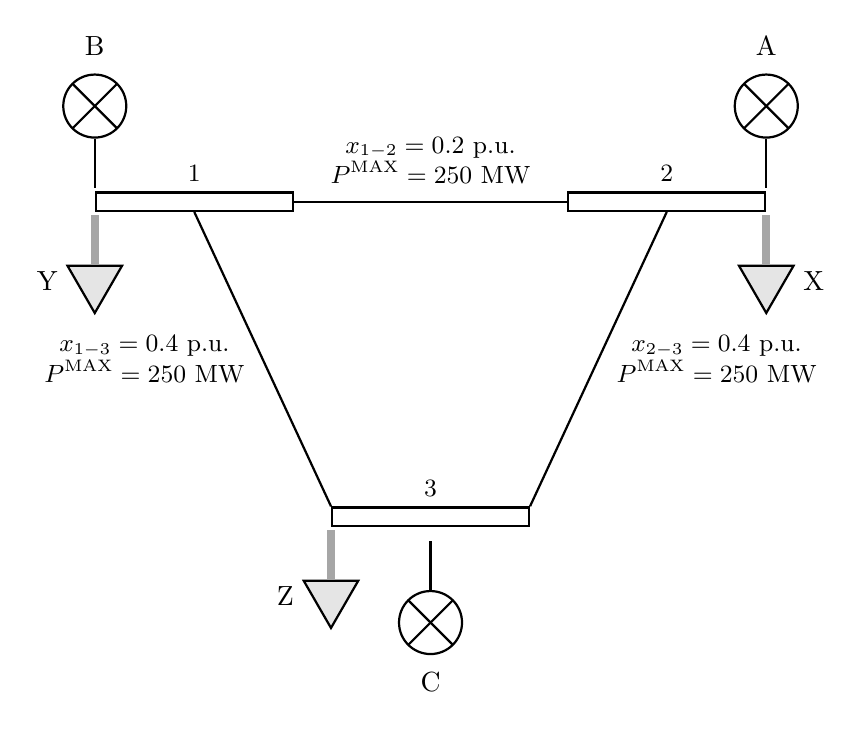
\begin{tikzpicture}
    % --- Nodes for Buses ---
    \node (bus1) [bus] at (0,0) {};
    \node[bus label] at (bus1.north) {1};
    \node (bus2) [bus] at (6,0) {};
    \node[bus label] at (bus2.north) {2};
    \node (bus3) [bus] at (3,-4) {};
    \node[bus label] at (bus3.north) {3};

    % --- Nodes for Generators ---
    \node (genB) [generator, above=0.8cm of bus1.west] {};
    \node[above=0.1cm of genB] {B};
    \node (genA) [generator, above=0.8cm of bus2.east] {};
    \node[above=0.1cm of genA] {A};
    \node (genC) [generator, below=0.8cm of bus3.south] {};
    \node[below=0.1cm of genC] {C};

    % --- Nodes for Loads ---
    \node (loadY) [load, below=0.8cm of bus1.west] {};
    \node[left=0.1cm of loadY] {Y};
    \node (loadX) [load, below=0.8cm of bus2.east] {};
    \node[right=0.1cm of loadX] {X};
    \node (loadZ) [load, below=0.8cm of bus3.west] {};
    \node[left=0.1cm of loadZ] {Z};

    % --- Transmission Lines ---
    \draw[line] (bus1.east) -- (bus2.west)
        node[midway, above=0.1cm, label style] {$x_{1-2} = 0.2 \text{ p.u.}$ \\ $P^{\text{MAX}} = 250 \text{ MW}$};
    \draw[line] (bus1.south) -- (bus3.north west)
        node[midway, left=0.1cm, label style] {$x_{1-3} = 0.4 \text{ p.u.}$ \\ $P^{\text{MAX}} = 250 \text{ MW}$};
    \draw[line] (bus2.south) -- (bus3.north east)
        node[midway, right=0.1cm, label style] {$x_{2-3} = 0.4 \text{ p.u.}$ \\ $P^{\text{MAX}} = 250 \text{ MW}$};

    % --- Connections ---
    \draw[line] (genB) -- ($(bus1.west) + (0,0.5em)$); 
    \draw[line] (genA) -- ($(bus2.east) + (0,0.5em)$); 
    \draw[line] (genC) -- ($(bus3.south) - (0,0.5em)$); 
    \draw[line, line width=3pt, gray!70] (loadY) -- ($(bus1.west) - (0,0.5em)$); 
    \draw[line, line width=3pt, gray!70] (loadX) -- ($(bus2.east) - (0,0.5em)$); 
    \draw[line, line width=3pt, gray!70] (loadZ) -- ($(bus3.west) - (0,0.5em)$); 
  \end{tikzpicture}
\end{center}

Now, to actually begin doing this problem...
\pagebreak

\subsection{Set 1}
We first have the following transactions:
\begin{itemize}
  \item B$\rightarrow$X: 200 MW
  \item A$\rightarrow$Z: 400 MW
  \item C$\rightarrow$Y: 300 MW
\end{itemize}
And now, with that, we can calculate the following... First is for $F_{12}$
\begin{alignat*}{1}
  F_{12} &= 200*\frac{0.8}{1} - 400*\frac{0.4}{1} - 300*\frac{0.4}{1} \\
  F_{12} &= 160 - 160 - 120 \\
  F_{12} &= -120\text{MW} < 250\text{MW} \cmark
\end{alignat*}
Now for $F_{23}$
\begin{alignat*}{1}
  F_{23} &= -200*\frac{0.2}{1} + 400*\frac{0.6}{1} - 300*\frac{0.4}{1} \\
  F_{23} &= -40 + 240 - 120 \\
  F_{23} &= 80\text{MW} < 250\text{MW} \cmark
\end{alignat*}
Now for $F_{13}$
\begin{alignat*}{1}
  F_{13} &= 200*\frac{0.2}{1} + 400*\frac{0.4}{1} - 300*\frac{0.6}{1} \\
  F_{13} &= 40 + 160 - 180 \\
  F_{13} &= 20\text{MW} < 250\text{MW} \cmark
\end{alignat*}
Due to all of this being below the 250MW, set 1 is all valid and feasible.

\subsection{Set 2}
For set 2, we have the following...
\begin{itemize}
  \item B$\rightarrow$Z: 600 MW
  \item A$\rightarrow$X: 300 MW
  \item A$\rightarrow$Y: 200 MW
  \item A$\rightarrow$Z: 200 MW
\end{itemize}
And when doing the same math we get the following...
\begin{alignat*}{1}
  F_{12} &= 600*\frac{0.4}{1} - 200*\frac{0.8}{1} - 200*\frac{0.4}{1} \\
  F_{12} &= 240 - 160 - 80 \\
  F_{12} &= 0\text{MW} < 250\text{MW} \cmark
\end{alignat*}
\begin{alignat*}{1}
  F_{13} &= 600*\frac{0.6}{1} - 200*\frac{0.2}{1} + 200*\frac{0.4}{1} \\
  F_{13} &= 360 - 40 + 80 \\
  F_{13} &= 400\text{MW} < 250\text{MW} \xmark
\end{alignat*}
\begin{alignat*}{1}
  F_{23} &= 600*\frac{0.4}{1} + 200*\frac{0.2}{1} + 200*\frac{0.6}{1} \\
  F_{23} &= 240 + 40 + 120 \\
  F_{23} &= 400\text{MW} < 250\text{MW} \xmark
\end{alignat*}
Due to all of this being above 250MW, set 2 is therefore invalid and not feasible.

\subsection{Set 3}
For set 3, we have the following...
\begin{itemize}
  \item C$\rightarrow$X: 1000 MW
  \item X$\rightarrow$Y: 400 MW
  \item B$\rightarrow$C: 300 MW
  \item A$\rightarrow$C: 200 MW
  \item A$\rightarrow$Z: 100 MW
\end{itemize}
And when doing the same math we get the following...
\begin{alignat*}{1}
  F_{12} &= 1000*\frac{0.4}{1} - 400*\frac{0.8}{1} + 300*\frac{0.4}{1}  - 200*\frac{0.4}{1} - 100*\frac{0.4}{1}\\
  F_{12} &= 80\text{MW} < 250\text{MW} \cmark
\end{alignat*}
\begin{alignat*}{1}
  F_{13} &= -1000*\frac{0.4}{1} - 400*\frac{0.8}{1} + 300*\frac{0.6}{1}  + 200*\frac{0.4}{1} + 100*\frac{0.4}{1}\\
  F_{13} &= -180\text{MW} < 250\text{MW} \cmark
\end{alignat*}
\begin{alignat*}{1}
  F_{23} &= -1000*\frac{0.6}{1} + 400*\frac{0.2}{1} + 300*\frac{0.4}{1}  + 200*\frac{0.6}{1} + 100*\frac{0.6}{1}\\
  F_{23} &= -220\text{MW} < 250\text{MW} \cmark
\end{alignat*}
Due to all of this being below 250MW, set 3 is therefore valid and feasible.

\pagebreak

\section{6.2}
\textbf{Given:} \textit{Consider the two-bus power system shown in the figure below. The marginal cost of production of the generators connected to buses A and B are given respectively also by the following expressions below:}
$$ MC_A = 20 + 0.03*P_A\frac{\$}{MWh} $$
$$ MC_B = 15 + 0.02*P_B\frac{\$}{MWh} $$

\begin{center}
  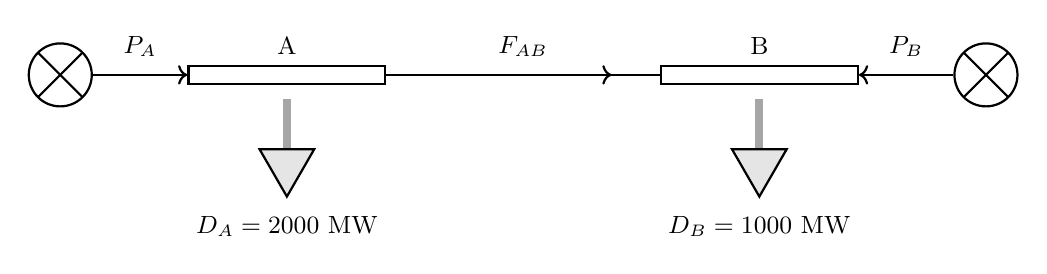
\begin{tikzpicture}
      % --- Nodes for Buses ---
      \node (busA) [bus] at (0,0) {};
      \node[bus label] at (busA.north) {A};
      \node (busB) [bus] at (6,0) {};
      \node[bus label] at (busB.north) {B};

      % --- Generators ---
      \node (genA) [generator, left=1.2cm of busA.west] {};
      \node (genB) [generator, right=1.2cm of busB.east] {};
      \draw[power_arrow] (genA.east) -- (busA.west) node[above=0.1cm, midway, font=\small] {$P_A$};
      \draw[power_arrow] (genB.west) -- (busB.east) node[above=0.1cm, midway, font=\small] {$P_B$}; 

      % --- Loads ---
      \node (loadA_shape) [load, below=0.8cm of busA.south] {};
      \draw[load_connector] ($(busA.south) - (0,0.5em)$) -- (loadA_shape.north);
      \node[below=0.1cm of loadA_shape.south, font=\small] {$D_A = 2000 \text{ MW}$};

      \node (loadB_shape) [load, below=0.8cm of busB.south] {};
      \draw[load_connector] ($(busB.south) - (0,0.5em)$) -- (loadB_shape.north);
      \node[below=0.1cm of loadB_shape.south, font=\small] {$D_B = 1000 \text{ MW}$};

      % --- Transmission Line ---
      \draw[line] (busA.east) -- (busB.west);
      \node (fab_label) at ($ (busA.east)!0.5!(busB.west) $) {}; 
      \draw[power_arrow] ($(fab_label.west)-(1cm,0)$) -- ($(fab_label.east)+(1cm,0)$)
          node[above=0.1cm, midway, font=\small] {$F_{AB}$};
  \end{tikzpicture}
\end{center}
\textit{Assume that the demand is constant and insensitive to price, that energy is sold at its marginal cost of production and that there are no limits on the output of the generators. calculate the price of electricity at each bus, the production each generator and the flow on the line for the following cases:}

\subsection{A. The line between buses A and B is disconnected.}
Since the line is disconnected we can assume that $F_{AB}=0$. Therefore, for bus A $P_A=D_A=2000$MW. And, when plugged into the price equation we get...
$$ \pi_A = MC_A = 20 + 0.03*(2000) = 80\frac{\$}{MWh} $$
And, now for bus B $P_B = D_B = 1000$MW. And, when plugged in like above we get....
$$ \pi_B = MC_B = 15 + 0.02*(1000) = 35\frac{\$}{MWh} $$

\subsection{B. The line between buses A and B is in service and has an unlimited capacity.}
Since the line here has unlimited capacity, we can safely assume that $F_{AB} = D_B - D_A$ (if we defined positive flow from B to A, but here standard convention is usually A to B, let's stick to the balance equations). With the total Demand, D, being $D = D_A + D_B = 3000$MW. Therefore, $P_B = 3000 - P_A$. Now, to find $P_A$, and also $P_B$, we have to do the following.
\begin{center}
  $$ MC_A = MC_B $$
  $$ 20 + 0.03*P_A = 15 + 0.02*P_B $$
  $$ 20 + 0.03*P_A = 15 + 0.02*(3000 - P_A) $$
  $$ 20 + 0.03*P_A = 15 + 60 - 0.02*P_A $$
  $$ 0.05*P_A = 55 $$
  $$ P_A = 1100MW $$
\end{center}
And so, therefore, $P_B = 1900MW$.
$$ \pi = MC_A = MC_B = 20 + 0.03*1100 = 53 \frac{\$}{MWh} $$
and therefore...
$$ F_{AB} = P_A - D_A = 1100 - 2000 = -900MW $$
(The negative sign implies 900 MW is flowing from B to A).

\subsection{C. The line between buses A and B is in service and has an unlimited capacity, but the maximum output of Generator B is 1500MW.}
From part (b), we saw that the optimal unconstrained dispatch for Generator B was 1900 MW. However, we are now limited to $P_B \le 1500$ MW. 
Since the optimal dispatch for B is higher than its limit, Generator B will run at its maximum capacity.
$$ P_B = 1500 \text{ MW} $$
Since total demand is 3000 MW:
$$ P_A = 3000 - 1500 = 1500 \text{ MW} $$
Since the line has unlimited capacity, there is a single market price. However, Generator B is at its limit and cannot supply the next increment of load. Generator A is the marginal unit.
$$ \pi = MC_A = 20 + 0.03(1500) = 65 \frac{\$}{MWh} $$
The flow on the line is:
$$ F_{AB} = P_A - D_A = 1500 - 2000 = -500 \text{ MW} $$

\subsection{D. The line between buses A and B is in service and has an unlimited capacity, but the maximum output of Generator A is 900MW.}
From part (b), the optimal unconstrained dispatch for Generator A was 1100 MW. Since the limit is 900 MW ($P_A \le 900$), Generator A is constrained and will run at its maximum.
$$ P_A = 900 \text{ MW} $$
Total demand is 3000 MW, so:
$$ P_B = 3000 - 900 = 2100 \text{ MW} $$
Generator B is now the marginal unit (it is unconstrained and picks up the slack).
$$ \pi = MC_B = 15 + 0.02(2100) = 57 \frac{\$}{MWh} $$
The flow on the line is:
$$ F_{AB} = P_A - D_A = 900 - 2000 = -1100 \text{ MW} $$

\subsection{E. The line between buses A and B is in service but its capacity is limited to 600MW. The output of the generators is unlimited.}
From part (b), the unconstrained flow was 900 MW from B to A ($F_{AB} = -900$). This violates the limit of 600 MW ($|F_{AB}| \le 600$).
Therefore, the line is congested, and the flow is fixed at the limit in the direction of the economic flow (from cheap B to expensive A).
$$ F_{AB} = -600 \text{ MW} $$
We can now solve for the generation at each bus using the power balance at each bus.
For Bus A:
$$ P_A - D_A = F_{AB} \implies P_A - 2000 = -600 \implies P_A = 1400 \text{ MW} $$
For Bus B:
$$ P_B - D_B = -F_{AB} \implies P_B - 1000 = 600 \implies P_B = 1600 \text{ MW} $$
Since the line is congested, the prices at the two buses uncouple.
$$ \pi_A = MC_A = 20 + 0.03(1400) = 62 \frac{\$}{MWh} $$
$$ \pi_B = MC_B = 15 + 0.02(1600) = 47 \frac{\$}{MWh} $$

\pagebreak

\section{6.3}
\textbf{Given:} \textit{Calculate the generator revenues and the consumer payments for all the cases considered in Problem 6.2. Who benefits from the line connecting these two buses?}

We define Generator Revenue ($R$) as $P_G \times \pi$ and Consumer Payments ($E$) as $D \times \pi$.

\textbf{Case A (Line Disconnected):}
$$ \pi_A = 80, \quad \pi_B = 35 $$
$$ R_A = 2000 \times 80 = \$160,000/h, \quad E_A = 2000 \times 80 = \$160,000/h $$
$$ R_B = 1000 \times 35 = \$35,000/h, \quad E_B = 1000 \times 35 = \$35,000/h $$

\textbf{Case B (Unlimited Line):}
$$ \pi = 53 $$
$$ R_A = 1100 \times 53 = \$58,300/h, \quad E_A = 2000 \times 53 = \$106,000/h $$
$$ R_B = 1900 \times 53 = \$100,700/h, \quad E_B = 1000 \times 53 = \$53,000/h $$

\textbf{Case C (Gen B Limited):}
$$ \pi = 65 $$
$$ R_A = 1500 \times 65 = \$97,500/h, \quad E_A = 2000 \times 65 = \$130,000/h $$
$$ R_B = 1500 \times 65 = \$97,500/h, \quad E_B = 1000 \times 65 = \$65,000/h $$

\textbf{Case D (Gen A Limited):}
$$ \pi = 57 $$
$$ R_A = 900 \times 57 = \$51,300/h, \quad E_A = 2000 \times 57 = \$114,000/h $$
$$ R_B = 2100 \times 57 = \$119,700/h, \quad E_B = 1000 \times 57 = \$57,000/h $$

\textbf{Case E (Line Capacity Limited):}
$$ \pi_A = 62, \quad \pi_B = 47 $$
$$ R_A = 1400 \times 62 = \$86,800/h, \quad E_A = 2000 \times 62 = \$124,000/h $$
$$ R_B = 1600 \times 47 = \$75,200/h, \quad E_B = 1000 \times 47 = \$47,000/h $$

\textbf{Analysis of Benefits:}
Comparing the connected cases to the disconnected case (Case A):
\begin{itemize}
    \item \textbf{Consumers at A:} Price drops from 80 (Case A) to 53 (Case B) or 62 (Case E). They benefit significantly from the line.
    \item \textbf{Consumers at B:} Price increases from 35 (Case A) to 53 (Case B) or 47 (Case E). They are worse off.
    \item \textbf{Generator A:} Price drops and production decreases. They are worse off.
    \item \textbf{Generator B:} Price increases and production increases (from 1000 to 1900 or 1600). They benefit significantly.
\end{itemize}
\textbf{Conclusion:} Generally, Generator B and Consumers at A benefit from the interconnection.

\section{6.4}
\textbf{Given:} \textit{Calculate the congestion surplus for the case (e) of Problem 6.2. Check your answer using the results of Problem 6.3. For what values of the flow on the line between buses A and B is the congestion surplus equal to zero?}

\textbf{Congestion Surplus Calculation:}
The congestion surplus (or merchandising surplus) is defined as the flow from B to A multiplied by the price difference between A and B.
$$ \text{Surplus} = (\pi_A - \pi_B) \times |F_{BA}| $$
$$ \text{Surplus} = (62 - 47) \times 600 = 15 \times 600 = \$9,000/h $$

\textbf{Check using Problem 6.3:}
The surplus should also equal the total payments by consumers minus the total revenue received by generators.
$$ \text{Total Payments} = E_A + E_B = 124,000 + 47,000 = \$171,000 $$
$$ \text{Total Revenue} = R_A + R_B = 86,800 + 75,200 = \$162,000 $$
$$ \text{Surplus} = 171,000 - 162,000 = \$9,000/h $$
The results match.

\textbf{Zero Congestion Surplus:}
The congestion surplus is zero when the price at Bus A equals the price at Bus B ($\pi_A = \pi_B$). 
This occurs when the transmission constraint is not binding. From Case (b), we know that the unconstrained flow is 900 MW.
Therefore, the congestion surplus is zero for any transmission capacity limit $\ge 900$ MW.

\end{document}
